% !Mode:: "TeX:UTF-8"

%%%中文版式与英文版式通过参数设置
\documentclass{ctacn}%英文版式

%可以选择使用times字体
\usepackage{newtxtext}
\usepackage{hhline}
\usepackage{ctex}

\begin{document}



%%%%%%%输入年、月、卷、期
\Volume{xxxx}{x}{xxx}{xx}{x}
\cndoi{1001-0920(0000)00-0000-00}
\doi{10.13195/j.kzyjc.0000.0000}
\paperdate{xxxx-xx-xx}{xxxx-xx-xx}%接收日期,修回日期
%%%%%%%设置开始页
\setcounter{page}{1}

%%%%%%%输入页眉显示的题目

%%%%%%%%%%
%%%                  本刊为匿名审稿,新投稿时不要填写任何作者信息,包括所有位置的姓名、单位以及邮箱
%%%%%%%%%%%%
\runheading{作者1~等: 控制与决策论文\LaTeX 模板说明}%页眉设置,填写第一作者及论文题目
\xiangmujijin{国家自然基金项目(00000000)}%项目基金  为空会自动取消显示
\authorintro{作者一\,(1974$-$), 男, 教授, 博士, 从事XXX及其应用等研究;作者(1990$-$), 男, 硕士生, 从事XXX的研究.}%作者简介,填写第一作者和导师的简介         %新投稿不修改
\authorcor{E-mail: zuozheyi@163.com}%通讯作者邮箱,新投稿不修改

%%%-------------中文信息---------------
\cntitle{控制与决策论文\LaTeX 模板说明 } %输入中文标题


%                  新投稿不要修改下面的姓名及单位
%%%中文作者和单位,\dag代表通信作者,“作者一”代表3个字的名,“作者”代表2个字的名
\cnauthor{作者一\makebox{$^{1,2\dag}$},~~作~~~~者\makebox{$^{1}$}}%新投稿不修改
{(1. 东北大学~信息科学与工程学院,沈阳~110004;2. 曲阜师范大学~工学院, 山东~日照~276826)}%%省会城市无需加省%%新投稿不要修改

%%%中文摘要
\cnabstract{本文给向《控制与决策》投稿的作者提供一个中文\LaTeX{}模版, 共分几章分别进行说明, 其中包括定理、定
义、推论等的引用; 公式的例子; 图形的插入; 表格的制作以及参考文献、作者简介等内容. 作者只需在相应的位置填
入相应的内容既可.}

%%%中文关键词
\cnkeyword{ 关键词1;关键词2;关键词3;关键词4}

%%%分类号、标识码
\clc{TP273}%中文分类号
\wenxianbiaoshi{A}%文献标志码

%%%%%%%----------------英文信息------------
\entitle{The Guide of the \LaTeX{} Template for preparing the manuscript of Control and Decision}


%%%%%%%              新投稿不要修改下面的英文名及单位
\enauthor{ZUO Zhe-yi\makebox{$^{1,2\dag}$},~~ZUO Zhe\makebox{$^{1}$}}{
(1. College of Information Science and Engineering,Northeastern University,Shenyang~110004,China;2. College of Engineering, Qufu Normal University,Rizhao~276826,China)}


\enabstract{ This article is designed to help in the contribution for Control and Decision. It is divided into several sections. It
consists of the styles and notes for the main text, the mathematical writing style and the topic of drawing tables and inserting
figures respectively. The residuals deal with references, acknowledges, etc.}

\enkeyword{Key word1;Key word2;Key word3;Key word4}

\maketitle




\begin{multicols}{2}
\section{引\quad  言}
本模版是新投稿模板.\;由于我刊是匿名审稿,任何位置的姓名、单位及邮箱都不要填写,

本模板所适用的编译环境是CTeX\,2.9.2.164和\linebreak TeXLive\,2015以后版本.

本模板可以使用以下两种方式编译:

 1. PDFLaTeX

2. XeLaTeX [推荐]


文中需特别说明的内容主要有以下几个方面:

摘要:摘要应体现目的、方法、结果和结论4要素,中文摘要以150\,$\sim$\,200字为宜,一般不用第一人称.

标题:一般的文章包含一级标题、二级标题甚至三级标题,例如:2;2.1;2.1.1等.

数学符号:文章中的数学符号,例如$x, y, Z$等.在以下的相关章节中会有
具体的公式例子.

插图:文中的插图要做到布局合理,尺寸适当,图形美观,线条清晰,文字符号简约.文中的图应以.eps的格式插入,且图中的有关说明应用中文,图名应该为中文形式且图的正下.

表格:表格结构应简洁、明确,尽量采用三线表(即:表格中没有竖线,只有三条横线(特殊情形除外),表名在表格的正上方.\;表中参量应标明单位.\;过长的表格可以通栏.

参考文献:文中引用的参考文献应是正式出版的图书、期刊、会议论文集等.\;文章中的参考文献的序号应该按正文中出现的先后顺序编排.


修改稿要求论点明确,论证充分,语句通顺,文字简练,字迹工整.定稿时论文不超过5页;短文不超过4页;综述与评论以及长论文字数可稍放宽.\;凡字数超过要求、文字不流畅、编排混乱的稿件不发表.

\section{应用环境}
应用如下的各种应用环境,定理、引理等自动生成,并按顺序生成编号.

% \begin{Thm}
% 	应用这个环境,定理编号将自动生成.
% \end{Thm}

% \begin{Site}
% 	应用这个环境,引理编号将自动生成.
% \end{Site}

% \begin{Cor}
% 	应用这个环境,推论编号将自动生成.
% \end{Cor}

% \begin{Def}
% 	应用这个环境,定义编号将自动生成.
% \end{Def}

% \begin{Sup}
% 	应用这个环境,假设编号将自动生成.
% \end{Sup}

% \begin{Exa}
% 	应用这个环境,例子编号将自动生成.
% \end{Exa}

% \begin{Stu}
% 	应用这个环境,情况编号将自动生成.
% \end{Stu}

% \begin{Exp}
% 	应用这个环境,实验编号将自动生成.
% \end{Exp}

% \begin{Sim}
% 	应用这个环境,仿真编号将自动生成.
% \end{Sim}

% \begin{Alg}
% 	应用这个环境,算法编号将自动生成.
% \end{Alg}

% \begin{Prop}
% 	应用这个环境,命题编号将自动生成.
% \end{Prop}

% \begin{Rem}
% 	应用这个环境,注编号将自动生成.
% \end{Rem}

证明的排版方式如下:

\textbf{证明}\quad 应用$\cdots$

证明成立. {\Large$\square$}

算法的步骤可以按如下排版.

1)\,大段落的内容:

\textbf{Step\,1}\quad
首先,假设$\cdots$.

\textbf{Step\,2}\quad
其次,证明$\cdots$.

\textbf{Step\,3}\quad
最后,得到$\cdots$.

2)\,小段落的内容:

Step\,1: $\cdots$;

Step\,2: $\cdots$;

Step\,3: $\cdots$.


\section{公式的例子}
\subsection{公式的应用环境}
公式请用环境\\
\verb|\begin{align}...\end{align}|
%有公式号
或者\\
\verb|\begin{align*}...\end{align*}|%没有公式号
\subsection{几个实例}

\subsubsection{公式分行的例子}
公式在符号后断开.
\begin{align}
{\Arrowvert x^{(1)}_{k+1}-x^{(1)}_k\Arrowvert}_\lambda\leqslant \;&
\frac{1}{1-h_1(i)}\Arrowvert x^{(1)}_{k+1}(0)-x^{(1)}_k(0)\Arrowvert+\notag\\
&\frac{h_2(i)}{1-h_1(i)}{\Arrowvert
	e^{(1)}_k\Arrowvert}_\lambda+\rho(Q).
\end{align}


\subsubsection{矩阵的例子}
1)\,矩阵中元素居中对齐;
\begin{align}
\left[\begin{array}{cccc}
a_{11}& a_{12}&\dots &a_{1n}\\
a_{21}& a_{22}&\dots &a_{2n}\\
\vdots&\vdots& \ddots   &\vdots\\
a_{n1}& a_{n2}&\dots &a_{nn}
\end{array}\right].\end{align}

2)\,两个公式左边对齐.
\begin{align}
&A_1=\left[\begin{array}{cc} 1& -2\\-2 &4
\end{array}\right],\\
&A_2=\left[\begin{array}{ccc} 1.1 &-2.7&-22.4\\-2.3 &4.6 &12.7
\end{array}\right].
\end{align}


\subsubsection{求最优值的例子}
只有一个公式号的情况,公式号放在最后;各约束条件左对齐.
\begin{align}
&\min~\alpha\sum\limits_{i=1}^n\xi_{i}T_{i}+\beta \sum\limits_{l=1}^m \varphi_{l} \max(\chi_{l},~0).\notag\\
&{\rm{~s.t.~}}T_{i}=\max(0,C_i-D_i),~\forall~i;\notag\\
&~~~~~~~~c_{i \delta k}-s_{i \delta k}=t_{i \delta k},~\forall~i,\delta,k;\notag\\
&~~~~~~~~s_{i 2 k}\geqslant c_{i 1 }+e_i,~\forall~i,k;\notag\\
&~~~~~~~~c_{j \delta' k'}-c_{i \delta k}+M(1-X_{i \delta k j\delta'k'})\geqslant t_{j \delta' k'},\notag\\
&~~~~~~~~~~~~~~~~~~~~~~~~~~\forall~i,j,\delta,\delta',k,k';\notag\\
&~~~~~~~~c_{i \delta k}-c_{j \delta' k'}+M X_{i \delta k j\delta'k'}\geqslant t_{i \delta k},\notag\\
&~~~~~~~~~~~~~~~~~~~~~~~~~~\forall~i,j,\delta,\delta',k,k';\notag\\
&~~~~~~~~|\min(\chi_{l},0)|\leqslant b_l,~\forall~ l;\notag\\
&~~~~~~~~\sum\limits_{l=1}^{l'-1} (b_{l}+\chi_{l})< \varepsilon_{\pi_{i \delta k}}\leqslant  \sum\limits_{l=1}^{l'} (b_{l}+\chi_{l}),~\pi_{i \delta k}=l;\notag\\
&~~~~~~~~X_{i \delta k j\delta'k'} \in {0,1},~\forall~ i,j,\delta,\delta',k,k'.
\end{align}


\subsubsection{带有大括号的例子}\vspace{-15pt}
\begin{align}
\left\{\begin{aligned}
&\dot{x}(t)=A_{i}x_{t}(0)+A_{i1}x_{t}(-r);\\
&y(t)=C_{i}x_{t}(0),t\geqslant t_{0}, i\in\{1, 2\}.
\end{aligned}\right.
\end{align}


\subsection{调整公式字体大小的特例}

用命令 \textbackslash displaystyle  可以调整在文字中过小的公式.\;$f(z)\thickapprox{\displaystyle\frac{1+\frac{1}{2}z+z^2+\frac{1}{2}z^3}{1-\frac{1}{2}z+z^2}}.$
类似前面这样的例子.

用命令 \textbackslash textstyle 可以调整公式中过大的情况.\;如下:
\begin{align}
&{\bm z}^{\rm T}(t)\{A_q^{\rm T}[P(t)+I]A_q-[P(t)+I]\}{\bm z}(t)+ \notag\\
&{\textstyle\bigcup\limits_{i=1}^m}\varint\nolimits_{t-\tau_i}^t{\bm
	z}^{\rm T}(s)\{A_q^{\rm T}A_q-I\}{\bm z}(s){\rm d}s\leqslant \notag\\
&{\bm z}^{\rm T}(t)\{A_q^{\rm T}[P(t)-I]A_q-[P(t)-I]\}{\bm z}(t)+ \notag\\
&{\textstyle\bigcup\limits_{i=1}^m}\varint\nolimits_{t-\tau_i}^t{\bm
	z}^{\rm T}(s)\{A_q^{\rm T}A_q-I\}{\bm z}(s){\rm d}s\leqslant 0.
\end{align}

\section{插~~~~~~图}

插图的格式为.eps,并利用下面的环境插入.图形的位置由命令
中“trim=0 0 0 0”来控制,可以通过修正其中的4个参数来移动图形的位置.
所给出的4个数字分别表示从图形的左边缘、下边缘、右边缘、上边缘被截去的值,
正数表示从边缘截去的大小, 而负数表示从边缘加上的大小.\;本刊为黑白出版,不同颜色的线条不易区分,请画成不同样式的线条.

1)\,框图必须有横纵坐标变量,有单位的变量提供单位,如图1所示.
\begin{center}
	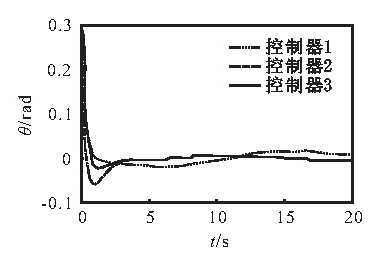
\includegraphics[scale=1,trim=0 0 0 0]{template-1}\\
	\label{Fig1}
	\figcaption{图形标题1}
\end{center}

2)\,流程图尽量简洁,步骤清楚,如图2所示.\vspace{10pt}
\begin{center}
	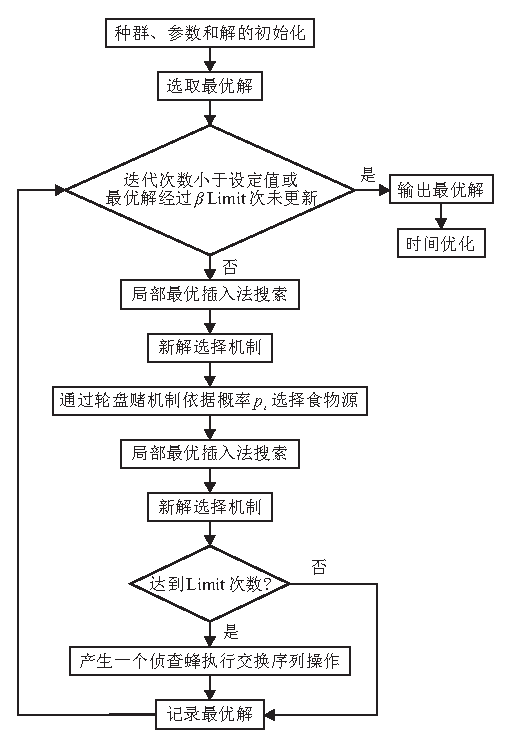
\includegraphics[scale=1,trim=0 0 0 0]{template-2}\\
	\label{Fig1}
	\figcaption{图形标题2}
\end{center}

3)\,图中有若干分图的必须有分图名,如图3所示.
\begin{center}
	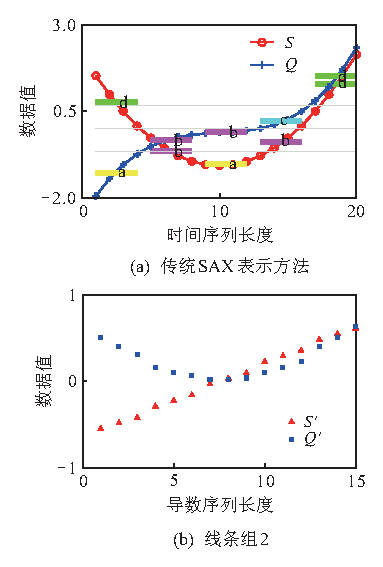
\includegraphics[scale=1,trim=0 0 0 0]{template-3}\\
	\label{Fig1}
	\figcaption{图形标题3}
\end{center}



\section{表~~~~~~格}
表格:表格结构应简洁、明确,尽量采用三线表(即:表格中没有竖线,只有三条横线(特殊情形除外),表名在表格的正上方.\;表中参量应标明单位.\;过长的表格可以通栏.

\begin{center}
	\tabcaption{二进制属性列$C_{i}$}
	\label{tab:1}
	\renewcommand\tabcolsep{10pt}
	\begin{tabular}{ccc||ccc}\toprule
		\multirow{2}{*}[-2pt]{$N$} &$C_1$ &$C_2$
		& \multirow{2}{*}[-2pt]{$N$} &$C_1$ &$C_2$ \\
		&$a$  &$b$     &    &$a$  &$b$  \\\hhline{---||---}
		1 & 1 & 0& $6$  & 1 & 1 \\
		2 & 1 & 0 &8 & 1 & 1 \\
		3 & 0 & 1 &9 & 1 & 1 \\
     	4 & 1 & 1 &10& 0 & 1 \\
		5 & 1 & 1 &11 & 0 & 1 \\
		6 & 1 & 1 &12& 0 & 1 \\
	    7 & 1 & 1 &13 & 0 & 1 \\
		\bottomrule
\end{tabular}\end{center}

\end{multicols}
\begin{center}
	\tabcaption{班组重构前后成本对比}
	\label{tab:1}
	\renewcommand\tabcolsep{10.6pt}%调整表格长度
	\begin{tabular}
{ccccccccc}\toprule
		%	\multirow{2}{1cm}[-2pt]{变量}......."{1cm}"代表这一栏目需要的长度;"[-2pt]"是为了让变量居中
		\multirow{2}{*}[-2pt]{$n$}&\multirow{2}{*}[-2pt]{$\alpha$} &\multirow{2}{*}[-2pt]{$\beta$}&\multicolumn{2}{c}{$f=1.5$} &\multirow{2}{*}[-2pt]{${\rm{Gap}}\%$}&\multicolumn{2}{c}{\multirow{1}{*}{$f=2$}} &\multirow{2}{*}[-2pt]{${\rm{Gap}}\%$}\\
		\cmidrule(lr){4-5}\cmidrule(lr){7-8}
		&&&重构&不重构&&重构&不重构\\\midrule
		&0.8&0.2&2\,140.6&4\,345.2&50.7&392.5&988.1&60.3\\
		$n=4$&0.5&0.5&1\,685.4&2\,717.0&38.0&143.1&215.3&33.5\\
		&0.2&0.8&944.5&1\,148.7&17.8&133.5&170.3&21.6\\\midrule
		&0.8&0.2&8\,865.7&16\,936.5&47.7&4\,949.9&10\,237.0&51.7 \\
		$n=6$&0.5&0.5&6\,264.6&10\,323.1&39.3&3\,232.4&6\,574.7&50.8\\
		&0.2&0.8&3\,110.8&4\,092.7&24.0&1\,943.7&2\,676.7&20.0\\
		\bottomrule
\end{tabular}\end{center}
\begin{multicols}{2}

\section{参考文献}
文章中的参考文献的序号应该按正文中出现的先后顺序编排(例如:因此这一控制方法已在控制理论领域引起了广泛的关注,其应用不仅
限于机器人控制领域\textsuperscript{[1-2]},而且在非线性系统的鲁棒
控制上也有了较大的发展\textsuperscript{[3-6]}.\;此外,在离散系统、分布参数系统上有了相应的应用\textsuperscript{[7-9]}.\;这一控制方法正逐步形成控制理论领域中的一个新方向,具体可以参见文献\textsuperscript{[10]}).\;同一处引用多篇文献,多篇文献置于一个方括号中;若多篇文献中没有连续的号,则各篇文献号之间用逗号;若多篇文献中即有不连续的,又有连续的号,则不连续的号之间用逗号,连续号之间用短连线,如[1,3-5].\;各类型参考文献的格式如下.

1)\,期刊文章:
[序号] 作者.\;文献题名[J].\;刊名,年,卷(期):起止页码.


2)\,图书:
[序号] 作者.\;文献题名[M].\;出版地:出版者,出版年:起止页码.

3)\,论文集:
[序号] 作者.\;文献题名[C].\;论文集名.\;出版地(指城市):出版者(或会议地点), 出版年:起止页码.

4)\,学位论文和学术报告:
[序号] 作者.\;文献题名[D或R].\;出版地(城市):出版者(单位),(出版)年份:起止页码.

5)\,国家标准:
[序号] 标准编号,标准名称[S].

6)\,专利:
[序号] 专利所有者.\;专利题名[P].\;国别:专利号.\;公告日期.

7)\,电子文档:
[序号] 主要责任者.\;题名[文献类型标志/文献载体标志].\;出版地:出版者, 出版年(更新或修改日期)[引用日期].\;获取和访问路径.

8)\,各种未定义类型的文献: [序号] 主要责任者.\;文献题名[Z].\;出版地(城市):出版者(单位),(出版)年份.

以上非英文文献者均需译成英文附在其后.


%%%%%%%%%%%%%%%%%%%%%%%%%%%%%%%%%%%%%%%%%%%%%%%%%%%%%%%%%%%%%%%%
%  参考文献
%%%%%%%%%%%%%%%%%%%%%%%%%%%%%%%%%%%%%%%%%%%%%%%%%%%%%%%%%%%%%%%%

\begin{thebibliography}{99}
  %段落之间的竖直距离
%1
%{\renewcommand{\baselinestretch}{1.02}\selectfont
\addtolength{\itemsep}{-0.7em}
\bibitem[1]{1}刘于之,李木国,杜海.\;具有时延和丢包的NCS鲁棒 $H_{\infty}$控制[J].\;控制与决策, 2014, 29(3): 517-522.\\
(Liu Y Z, Li M G, Du H. Robust $H_{\infty}$ control of NCS with delay and packet dropout[J]. Control and Decision, 2014, 29(3): 517-522.)
%2
\bibitem[2]{2}Zhu X L, Yue D. Stability of sampled-data systems with application to networked control systems[C]. Proc of the 32nd Chinese Control Conf. Xi'an: IEEE, 2013: 6572-6577.
%3
\bibitem[3]{3}Zhang C K, Jiang L, He Y, et al. Stability analysis for control systems with aperiodically sampled data using an augmented Lyapunov functional method[J]. IET Control Theory and Applications, 2013, 7(9): 1219-1226.
%4
\bibitem[4]{4}Seuret A, Briat C, Gouaisbaut F. Stability analysis of asynchronous sampled-data systems with discrete-time constant input delay[C]. Proc of the 53rd IEEE Conf on Decision and Control. Los Angeles: IEEE, 2014: 4342-4347.
%5
\bibitem[5]{5}Fujioka H. A discrete-time approach to stability analysis of systems with aperiodic sample-and-hold devices[J]. IEEE Trans on Automatic Control, 2009, 54(10): 2440-2445.
%6
\bibitem[6]{6}Naghshtabrizi P, Hespanha J P, Teel A R. Exponential stability of impulsive systems with application to uncertain sampled-data systems[J].  Systems \&  Control Letters, 2008, 57(5): 378-385.
%7
\bibitem[7]{7}Fridman E. A refined input delay approach to sampled-data control[J].  Automatica, 2010, 46(2): 421-427.
%8
\bibitem[8]{8}Liu K, Fridman E. Wirtinger's inequality and Lyapunov-based sampled-data stabilization[J].  Automatica, 2012, 48(1): 102-108.
%9
\bibitem[9]{9}Shao H Y, Han Q L, Zhang Z Q, et al. Sampling-interval-dependent stability for sampled-data systems with state quantization[J].  Int J of Robust Nonlinear Control, 2014, 24(17): 2995-3008.
%10
\bibitem[10]{10}Shao H Y, Lam J, Feng Z G. Sampling-interval-dependent stability for linear sampled-data systems with non-uniform sampling[J]. Int J of Systems Science, 2016, 47(12): 2893-2900.
%11
\bibitem[11]{11}Seuret A. A novel stability analysis of linear systems under asynchronous samplings[J]. Automatica, 2012, 48(1): 177-182.
%12
\bibitem[12]{12}Seuret A, Gouaisbaut F. Wirtinger-based integral\linebreak     inequality: Application to time-delay systems[J]. Automatica, 2013, 49(9): 2860-2866.
%13
\bibitem[13]{13}Gu K. An integral inequality in the stability problem of time-delay systems[C]. Proc of the 39th IEEE Conf on Decision and Control. Sydney: IEEE, 2000: 2805-2810.

\end{thebibliography}\vspace{-20pt}
\editor{X~~~~X}
\end{multicols}
\end{document}
